\documentclass[conference]{IEEEtran}
\IEEEoverridecommandlockouts
% The preceding line is only needed to identify funding in the first footnote. If that is unneeded, please comment it out.
\usepackage{cite}
\usepackage{amsmath,amssymb,amsfonts}
\usepackage{algorithmic}
\usepackage{graphicx}
\usepackage{textcomp}
\usepackage{xcolor}
\usepackage{enumitem}
\usepackage{float}
\def\BibTeX{{\rm B\kern-.05em{\sc i\kern-.025em b}\kern-.08em
    T\kern-.1667em\lower.7ex\hbox{E}\kern-.125emX}}
\begin{document}

\title{A Study on Explainability in RL Models\\
}

\author{\IEEEauthorblockN{Joseph (Jack) Bosco}
\IEEEauthorblockA{\textit{dept. name} \\
\textit{Columbia University}\\
New York, NY \\
jab2516}
\and
\IEEEauthorblockN{Akshara Pramod}
\IEEEauthorblockA{\textit{School of Engineering and Applied Science} \\
\textit{Columbia University}\\
New York, NY \\
ap4613} 
}


\maketitle

\begin{abstract}
This project explores the application of Variational Autoencoders (VAEs) to enhance explainability in reinforcement learning (RL) models applied to the CarRacing-v3 environment. We propose and implement a framework that learns meaningful low-dimensional latent representations from high-dimensional visual inputs, enabling more interpretable and efficient training of RL agents. By training a VAE on frames collected from human gameplay and then using the encoded latent space as the state representation for a Soft Actor-Critic (SAC) agent, we create an architecture that bridges the explainability gap in deep RL systems. Our approach demonstrates how dimensionality reduction through VAEs creates interpretable state representations while maintaining performance. We utilize t-SNE visualization, latent space traversal, policy vector field analysis, and cluster analysis to gain insights into the agent's decision-making process. Results show that our 2-dimensional latent space effectively captures essential driving features and enables visualization of the agent's policy, proving the value of this approach for explainability in high-dimensional RL tasks.
\end{abstract}

\begin{IEEEkeywords}
VAE, Soft Actor-Critic Agent (SAC), Deep RL
\end{IEEEkeywords}

\section{Introduction}
Deep reinforcement learning has achieved remarkable success in solving complex tasks, particularly in environments with high-dimensional sensory inputs such as image data. However, most deep RL models operate as black boxes, making it challenging to interpret why certain decisions are made. This lack of transparency poses significant challenges for stakeholders who must trust these automated systems, especially in safety-critical domains like autonomous driving.


The ability to explain AI decisions is increasingly recognized as essential for real-world deployment, as emphasized by regulatory frameworks like the EU's General Data Protection Regulation (GDPR), which includes a "right to explanation" for automated decisions. This is particularly relevant for high-stakes domains where human safety may be at risk.

In this project, we address the explainability challenge in RL by incorporating Variational Autoencoders to learn meaningful latent representations from high-dimensional visual states in the CarRacing-v3 environment. Our approach brings two key advantages: (1) learning a compressed, meaningful state representation that captures essential driving features and (2) enabling interpretable visualization of the agent's decision-making process.

We aim at demonstrating that a low-dimensional latent space (just 2 dimensions) can effectively capture the essential features needed for performing well in a driving task while simultaneously enabling visualization and interpretation of the agent's policy. This represents a significant step toward explainable RL systems that can be trusted and understood by human operators.

\section{Related Work}

\subsection{To be Added}


\section{Methods}
\begin{figure}[H]
    \centering
    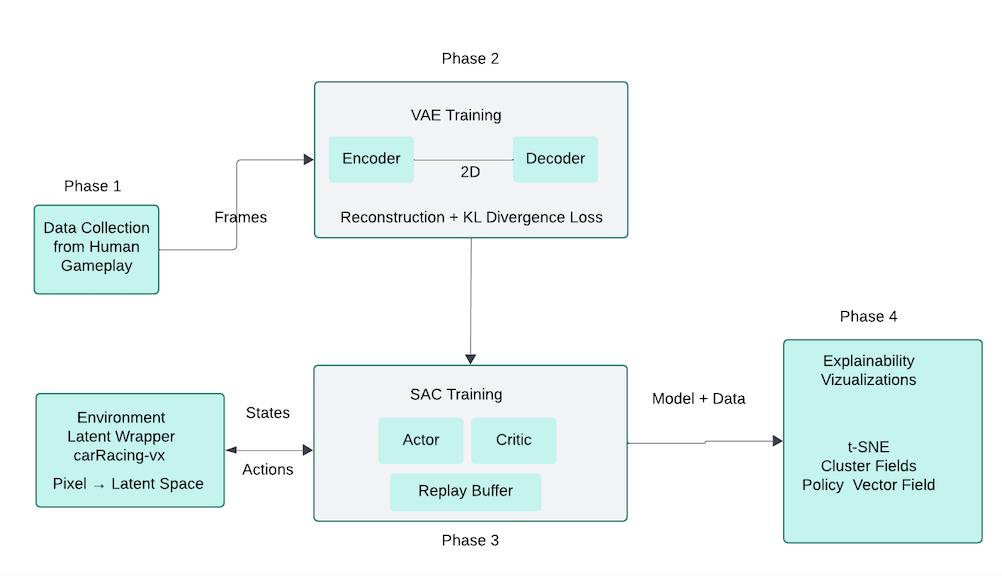
\includegraphics[width=0.75\linewidth]{Writeup/system-overview.png}
    \caption{System Workflow}
    \label{fig:System Architecture}
\end{figure}

Our approach integrates three key components to create an explainable reinforcement learning system:

\begin{enumerate}[label=\roman*.]
    \item \textbf{Variational Autoencoder (VAE) for learning interpretable state representations:} A deep generative model that compresses high-dimensional visual inputs (96$\times$96$\times$3 RGB images) into a structured 2-dimensional latent space, capturing essential driving features while enabling direct visualization.
    
    \item \textbf{Soft Actor-Critic (SAC) algorithm for policy learning:} A maximum entropy reinforcement learning algorithm that learns a driving policy directly in the VAE's latent space, balancing exploration and exploitation while effectively handling the continuous control task of steering and acceleration.
    
    \item \textbf{Specialized visualization techniques for explainability:} A suite of complementary methods including policy vector field visualization, t-SNE embedding, cluster analysis, and trajectory tracking that reveal different aspects of the agent's decision-making process and behavioral patterns.
\end{enumerate}

This section provides the theoretical foundations and conceptual understanding of each component.

\subsection{Framework Overview}

Deep reinforcement learning systems operating on high-dimensional inputs such as images typically function as black boxes, with internal representations that resist human interpretation. Our framework addresses this explainability challenge by decomposing the learning process into sequential stages. First, we learn a compressed, structured representation of the visual environment using a VAE. Then, we train a reinforcement learning agent directly in this interpretable latent space rather than on raw pixels. Finally, we apply visualization techniques to reveal the agent's decision-making process.

This decomposition provides two crucial advantages: it creates an inherently more interpretable state representation, and it simplifies the reinforcement learning task by reducing its dimensionality. Figure 1 illustrates the overall architecture of our approach.

\subsection{Variational Autoencoders: Theoretical Foundations}

Variational Autoencoders represent a class of generative models that learn compact latent representations of high-dimensional data through a principled probabilistic framework. Unlike standard autoencoders that deterministically map inputs to latent codes, VAEs model the underlying probability distribution of the data, enabling more robust representations and generative capabilities.

\subsubsection{Probabilistic Formulation}

The VAE framework models the data generation process as involving latent variables $z$ that generate observable variables $x$ through some conditional distribution $p_\theta(x|z)$. The joint distribution $p(x,z)$ is factorized as:

\begin{equation}
p(x,z) = p(z)p_\theta(x|z)
\end{equation}

Where $p(z)$ is typically a standard normal distribution $\mathcal{N}(0,I)$.

The key challenge in VAEs is inference—computing the posterior distribution $p(z|x)$, which is generally intractable. VAEs address this by introducing an approximate posterior $q_\phi(z|x)$ parameterized by neural networks, and then optimizing the parameters to minimize the difference between the true and approximate posteriors.

\subsubsection{Evidence Lower Bound}

VAEs are trained to maximize the Evidence Lower Bound (ELBO):

\begin{equation}
\mathcal{L}(\theta, \phi; x) = \mathbb{E}_{q_\phi(z|x)}[\log p_\theta(x|z)] - D_{KL}(q_\phi(z|x) \| p(z))
\end{equation}

The first term represents the reconstruction quality—how well the decoder can reconstruct the input from the latent code. The second term is the Kullback-Leibler divergence between the approximate posterior and the prior, serving as a regularization term that encourages the latent space to have a structured distribution.

In our work, the VAE serves as a state abstraction mechanism that compresses the high-dimensional visual input from the CarRacing environment into a low-dimensional space that captures the essential driving features while enabling direct visualization.

\subsection{Soft Actor-Critic: Theoretical Foundations}

Soft Actor-Critic is a state-of-the-art deep reinforcement learning algorithm based on the maximum entropy framework, which augments the standard RL objective with an entropy maximization term. This approach leads to more robust policies that explore more effectively and can better handle uncertainty.

\subsubsection{Maximum Entropy Objective}

The standard RL objective seeks to maximize expected cumulative rewards:

\begin{equation}
J(\pi) = \mathbb{E}_{\pi}\left[\sum_{t=0}^{\infty} \gamma^t r(s_t, a_t)\right]
\end{equation}

SAC extends this with an entropy term to form the maximum entropy objective:

\begin{equation}
J(\pi) = \mathbb{E}_{\pi}\left[\sum_{t=0}^{\infty} \gamma^t \left(r(s_t, a_t) + \alpha \mathcal{H}(\pi(\cdot|s_t))\right)\right]
\end{equation}

Where $\mathcal{H}(\pi(\cdot|s_t))$ represents the entropy of the policy at state $s_t$, and $\alpha$ is a temperature parameter controlling the trade-off between reward maximization and entropy maximization.

\subsubsection{Actor-Critic Architecture}

SAC employs an actor-critic architecture with several key components:

\begin{enumerate}[label=\roman*.]
    \item A policy network (actor) $\pi_\phi(a|s)$ that outputs a distribution over actions
    \item Twin Q-networks (critics) $Q_{\theta_1}(s,a)$ and $Q_{\theta_2}(s,a)$ that estimate expected returns
    \item A temperature parameter $\alpha$ that balances exploration and exploitation
\end{enumerate}

The critics are trained to minimize the Bellman error, while the actor is trained to maximize the expected Q-value while maintaining high entropy:

\begin{equation}
J_\pi(\phi) = \mathbb{E}_{s \sim \mathcal{D}}\left[\mathbb{E}_{a \sim \pi_\phi(\cdot|s)}\left[Q_\theta(s,a) - \alpha \log \pi_\phi(a|s)\right]\right]
\end{equation}


In our framework, SAC learns directly in the VAE's latent space, taking advantage of the compact, structured representation to learn effective driving policies more efficiently while maintaining interpretability.

\subsection{Explainability Methods: Theoretical Foundations}

Explainable AI (XAI) methods seek to make AI systems' decision-making processes transparent and interpretable to humans. In reinforcement learning, explainability is particularly challenging due to the sequential nature of decision-making and the complexity of the learned policies.

\subsubsection{Approaches to RL Explainability}

Explainable reinforcement learning typically employs one or more of the following approaches:

\begin{enumerate}[label=\roman*.]
    \item \textbf{State space visualization}: Techniques that visualize the agent's state representation, revealing how it perceives and organizes the environment.
    
    \item \textbf{Policy visualization}: Methods that illustrate how the agent maps states to actions, revealing its decision-making strategies.
    
    \item \textbf{Trajectory analysis}: Approaches that examine complete sequences of states and actions, showing how decisions unfold over time.
    
\end{enumerate}

\subsubsection{Dimensionality Reduction and Clustering}

Two foundational techniques for explainability are dimensionality reduction and clustering:

\begin{enumerate}[label=\roman*.]
    \item \textbf{Dimensionality reduction}: Methods like t-SNE (t-distributed Stochastic Neighbor Embedding) project high-dimensional data into lower-dimensional spaces while preserving local structure. t-SNE minimizes the divergence between probability distributions that represent similarities in the original and reduced spaces, making it particularly effective at revealing clusters.
    
    \item \textbf{Clustering}: Techniques like K-means partition the state space into distinct groups based on similarity, revealing behavioral modes in the agent's strategy. K-means minimizes the sum of squared distances between points and their assigned cluster centers.
\end{enumerate}

\subsubsection{Vector Fields and Trajectory Analysis}

For understanding policies and behaviors over time, vector fields and trajectory analysis provide powerful tools:

\begin{enumerate}[label=\roman*.]
    \item \textbf{Vector fields}: Visualizations that show the agent's action at every point in the state space, revealing the flow of the policy. These are analogous to force fields in physics, showing how the agent would act from any possible state.
    
    \item \textbf{Trajectory analysis}: The study of state-action sequences over time, revealing how the agent navigates through the state space. This approach draws from dynamical systems theory, where phase portraits show how systems evolve.
\end{enumerate}

In our framework, these explainability methods transform the traditionally opaque deep RL system into a transparent one, where the agent's perceptions, decisions, and strategies can be directly observed and analyzed.

\section{Experiments}
\subsection{Dataset Collection and Preprocessing}

We collected a comprehensive dataset specifically for training our VAE model. This dataset consisted of 2,000 RGB frames with dimensions $96 \times 96 \times 3$ captured from human gameplay sessions in the CarRacing-v3 environment. Human gameplay was selected over random exploration to ensure the dataset contained meaningful driving behaviors that would be encountered during actual policy execution.

\subsubsection{Data Acquisition Process}
The data collection process involved:
\begin{enumerate}[label=\roman*.]
    \item Recording approximately 10 complete human gameplay episodes using the Gymnasium render functionality
    \item Sampling frames at regular intervals (every 3 timesteps) to ensure diversity while maintaining temporal coherence
    \item Storing raw frames as PNG files to preserve image quality
    \item Ensuring coverage of various track configurations, turn types, and driving scenarios
\end{enumerate}

\subsubsection{Data Augmentation}
To enhance the diversity and robustness of our training dataset, we implemented the following augmentation techniques:
\begin{enumerate}[label=\roman*.]
    \item \textbf{Region-specific cropping:} We identified that pixels 0-83 contained the static toolbar in the CarRacing environment. This region was cropped to focus the model on the dynamic driving area.
    
    \item \textbf{Horizontal flipping:} We applied horizontal mirroring only to the relevant gameplay region above the toolbar. This effectively doubled our dataset size while creating balanced representations of left and right turning scenarios, which is critical for learning symmetrical driving behaviors.
\end{enumerate}

These augmentation techniques expanded our effective dataset size to approximately 4,000 frames, providing sufficient variety for the VAE to learn a robust latent representation.

\subsubsection{Preprocessing Pipeline}
Our preprocessing pipeline consisted of the following steps:
\begin{enumerate}[label=\roman*.]
    \item Conversion from RGB to normalized floating-point tensors in range [0,1]
    \item Application of augmentation techniques
    \item Construction of a PyTorch \texttt{Dataset} class with custom transformations
    \item Creation of data loaders with batch size 64 for efficient training
\end{enumerate}

The dataset was partitioned using \texttt{torch.utils.data.random\_split} with fixed random seeds (42) to ensure reproducibility:
\begin{enumerate}[label=\roman*.]
    \item 80\% training set (approximately 3,200 augmented frames)
    \item 10\% validation set (approximately 400 augmented frames)
    \item 10\% test set (approximately 400 augmented frames)
\end{enumerate}

\subsection{VAE Training}

Our VAE implementation used a convolutional architecture specifically designed for the CarRacing environment, as demostrated in the figure 2 below.
\begin{figure}[H]
    \centering
    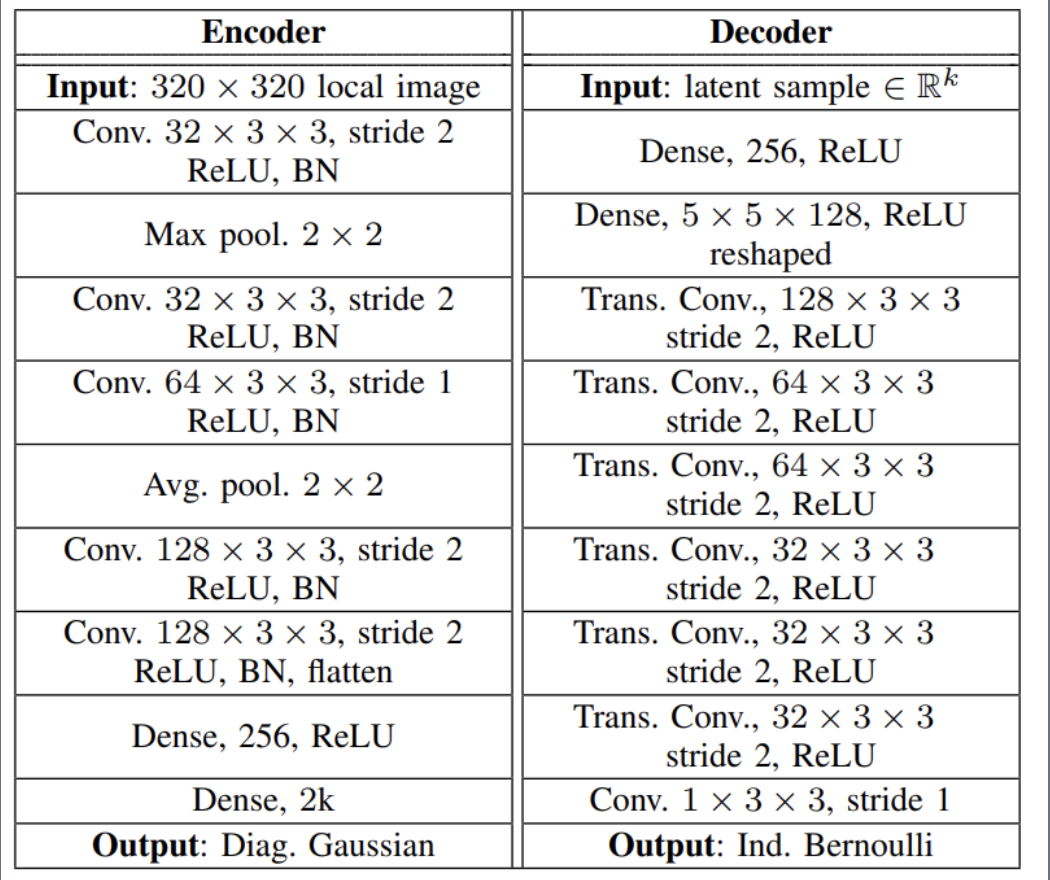
\includegraphics[width=0.75\linewidth]{Writeup/vae-arch.png}
    \caption{VAE Architecture}
    \label{fig:enter-label}
\end{figure}

\subsubsection{Implementation Details}
We implemented the VAE in PyTorch 1.x and optimized it using Adam optimizer with learning rate $1 \times 10^{-3}$ and momentum parameters $\beta_1 = 0.9$, $\beta_2 = 0.999$. The model was trained for 200 epochs with batch size 64. To ensure reproducibility and track progress, model weights were checkpointed every 20 epochs. We displayed early validation reconstructions periodically during training to monitor for potential overfitting and ensure the model was learning meaningful representations.

The BatchNorm2d layers after convolutional operations were critical for training stability, especially given the relatively small dataset size. The pooling operations helped reduce spatial dimensions efficiently while maintaining feature representation quality.

\subsubsection{Rationale for Pretraining}
By learning an unsupervised world model of the CarRacing frames, we were able to extract features that capture essential track geometry and car orientation [2]. These compact latent features greatly reduce the state dimensionality for the downstream RL agent, from the original 27,648 dimensions (96×96×3) to just 2 dimensions.

This approach offered two key advantages: First, it significantly improved sample efficiency for reinforcement learning by providing a structured, low-dimensional state space. Second, it enabled direct interpretability of the agent's behavior by creating a visualizable representation of the environment state. As demonstrated by White [7], such latent representations can be highly effective for understanding how generative models conceptualize their environment.

\subsection{Environment Wrapper}

To integrate the trained VAE with the reinforcement learning agent, we developed a custom wrapper for the CarRacing-v3 environment:

\begin{itemize}
    \item \textbf{LatentPassthroughExtractor:} A feature extractor class compatible with Stable Baselines3 that passes the latent vectors directly to the policy network without further processing.
    
    \item \textbf{CarRacingLatentWrapper:} A Gymnasium wrapper that encodes RGB observations through the VAE encoder before passing them to the agent and implements reward shaping.
\end{itemize}

\subsection{SAC Training}

We implemented the Soft Actor-Critic algorithm using the Stable Baselines3 library with several customizations:

\subsubsection{Environment Setup}
\begin{itemize}
    \item Base environment: CarRacing-v3 with no rendering during training
    \item Wrapper: CarRacingLatentWrapper with our pre-trained VAE
    \item RecordEpisodeStatistics wrapper for performance tracking
    \item DummyVecEnv for compatibility with Stable Baselines3
    \item VecNormalize for observation and reward normalization
\end{itemize}

\subsubsection{Policy Configuration}
\begin{itemize}
    \item Policy type: MlpPolicy
    \item Feature extractor: LatentPassthroughExtractor
    \item Network architecture: 2 hidden layers with 256 units each
    \item Activation function: ReLU
    \item Output distribution: Gaussian with state-dependent mean and standard deviation
\end{itemize}

\subsubsection{Training Hyperparameters}
We initialized the SAC agent with carefully tuned parameters for our specific task:

\begin{verbatim}
model = SAC(
    "MlpPolicy",
    venv,
    policy_kwargs=policy_kwargs,
    learning_rate=3e-4,
    buffer_size=200_000,
    batch_size=256,
    tau=0.005,
    gamma=0.99,
    train_freq=1,
    gradient_steps=1,
    verbose=1,
    device="cuda" if torch.cuda.is_available() 
    else "cpu" #NVIDIA T4 GPU used
)
\end{verbatim}

\subsubsection{Evaluation and Checkpointing}
\begin{itemize}
    \item Evaluation frequency: Every 20,000 timesteps
    \item Number of evaluation episodes: 5
    \item Evaluation deterministic: True (using mean action)
    \item Checkpoint saving frequency: Every 100,000 timesteps
    \item Best model saving: Based on mean evaluation reward
\end{itemize}

The SAC agent was trained for a total of 1,000,000 timesteps, which took approximately 8 hours on our hardware setup. We monitored training progress using TensorBoard logs, tracking episode rewards, episode lengths, and policy entropy.

\subsection{Explainability Analysis}

\subsubsection{Data Collection}
For our explainability analysis, we collected 5,000 state-action pairs from the trained agent. We created a testing environment with the pre-trained VAE and loaded the best SAC model identified during training. For each interaction, we recorded the 2D latent state vector, agent's actions (steering and acceleration), critic's Q-value estimates, rewards received, and termination flags. This comprehensive dataset provided the foundation for our visualization techniques.

\subsubsection{T-SNE Visualization}
We applied t-SNE dimensionality reduction (perplexity=30, 3,000 iterations) to visualize relationships between states and actions. Four visualizations were created using the same embedding but with different coloring schemes: steering actions (coolwarm colormap), acceleration values (viridis colormap), estimated Q-values (plasma colormap), and rewards (RdYlGn colormap). These visualizations revealed how different state regions correspond to specific driving behaviors and value estimates.

\subsubsection{Cluster Analysis}
K-means clustering (k=5) was applied to identify distinct behavioral modes in the latent space. For each cluster, we calculated mean steering and acceleration values to determine the characteristic behavior represented. The analysis revealed specialized clusters for different driving maneuvers: left turns, right turns, straightaways, and transitional states. This clustering provided an interpretable taxonomy of the agent's behavioral repertoire.

\subsubsection{Policy Vector Field}
We created a comprehensive policy visualization by sampling the agent's actions across a uniform 20×20 grid spanning the latent space (-3 to +3 in both dimensions). At each point, we queried both the policy and critic networks to obtain actions and value estimates. The resulting vector field visualization used steering values to determine flow direction and Q-values for coloring, with matplotlib's streamplot function rendering the field. This visualization revealed the global structure of the agent's policy across the entire state space.

\subsubsection{Trajectory Visualization}
We recorded three complete episodes in the latent space to understand the agent's temporal behavior. Each episode trajectory was plotted with a distinct color, with special markers for starting and ending points. Background points representing previously explored states provided context for the trajectories. This visualization revealed how the agent chains behaviors over time, showing cyclical patterns corresponding to lap completion and transitions between different driving modes.

\section{Results}

\subsection{Agent Performance}

Our SAC agent, trained on the 2-dimensional latent representation, achieved impressive performance in the CarRacing environment. During final evaluation, the agent demonstrated:

\begin{table}[h]
\centering
\caption{Agent Performance Metrics}
\begin{tabular}{|l|c|}
\hline
\textbf{Metric} & \textbf{Value} \\
\hline
Average Reward & $997.43 \pm 64.79$ \\
\hline
Min/Max Reward & $910.61 / 1066.22$ \\
\hline
Average Episode Length & $1000.00$ steps (maximum) \\
\hline
Average Tiles Visited & $224.67$ \\
\hline
\end{tabular}
\label{tab:performance}
\end{table}

This performance confirms that our 2D latent representation captured sufficient information for effective driving. The agent consistently completed tracks with high rewards, approaching the theoretical maximum score of around 1000.

\subsection{Latent Policy Analysis}
\begin{figure}
    \centering
    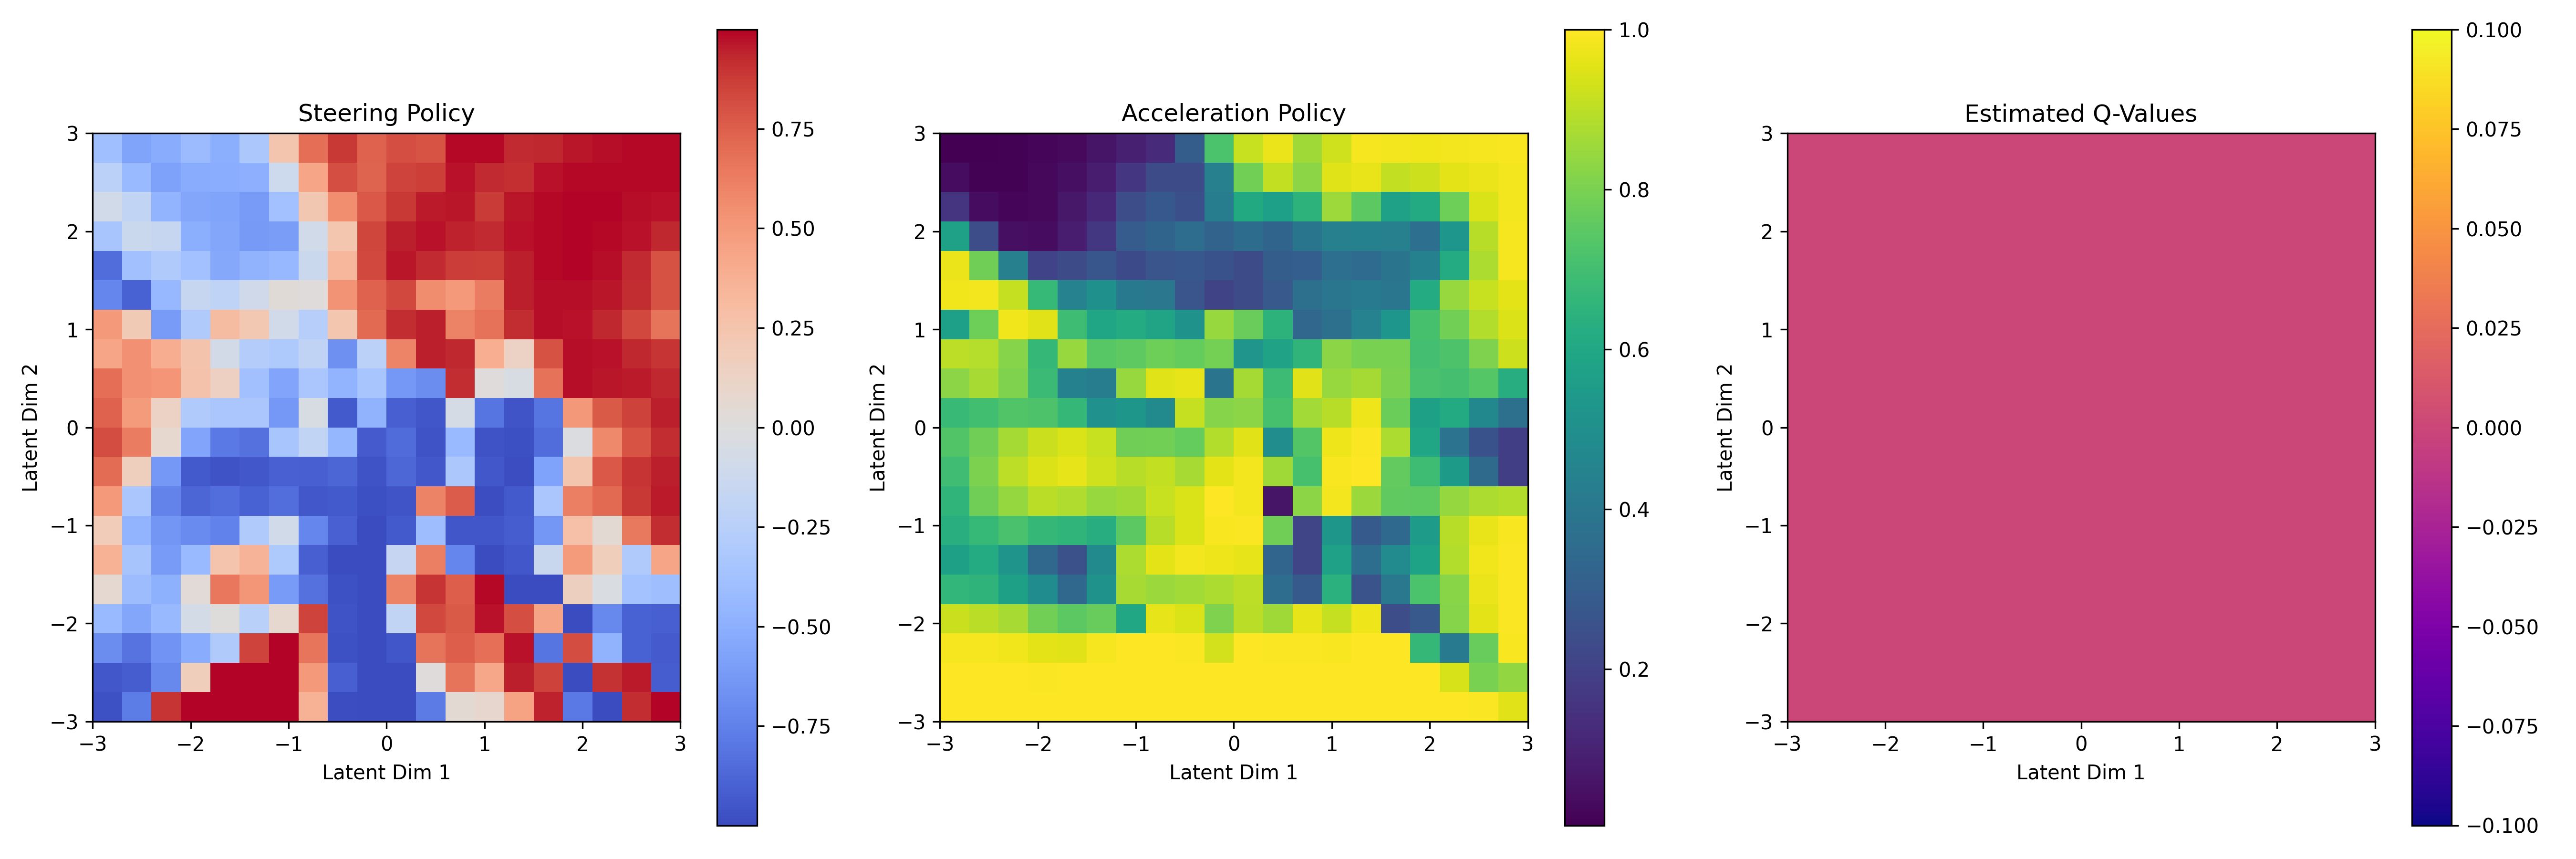
\includegraphics[width=0.75\linewidth]{Writeup/latent-grid.png}
    \caption{Latent Policy Analysis Grid}
    \label{fig:enter-label}
\end{figure}
\begin{figure}
    \centering
    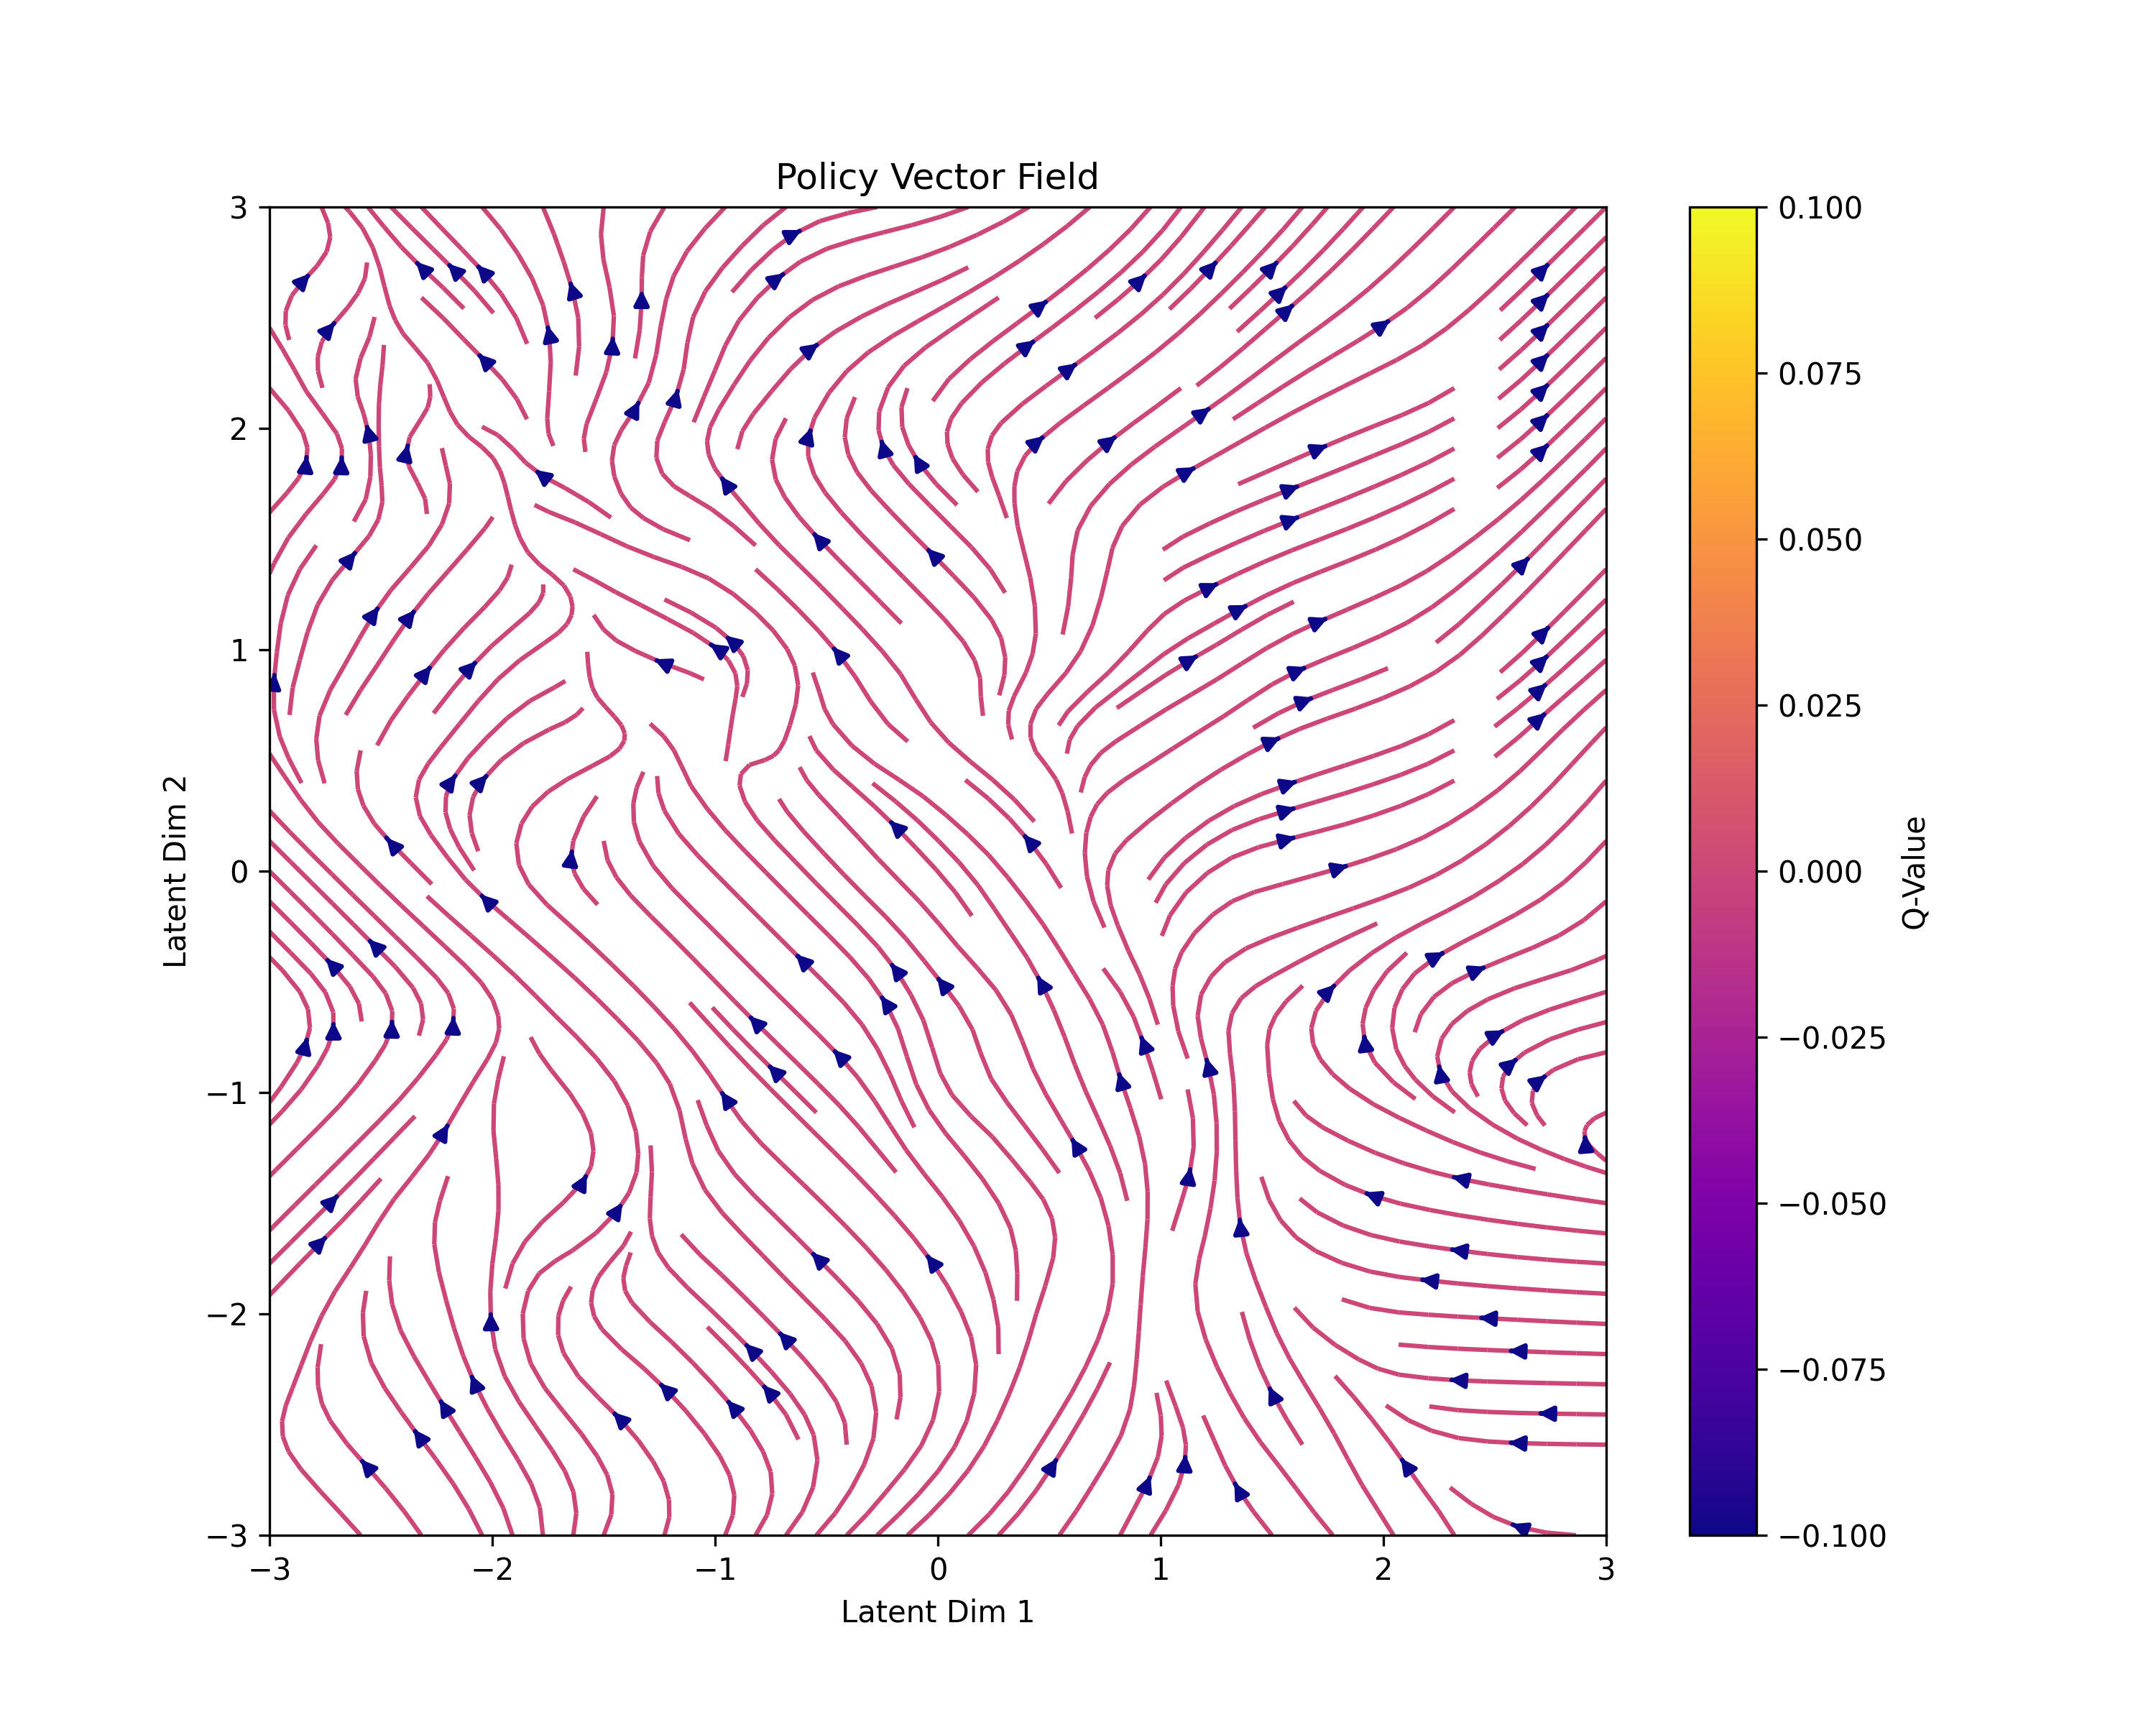
\includegraphics[width=0.75\linewidth]{Writeup/policy-vector-field.png}
    \caption{Policy Vector Field}
    \label{fig:enter-label}
\end{figure}
Figure 3 displays the learned policy structure across the latent space through three complementary visualizations. The steering policy (left) shows a clear separation between left-turning regions (blue) and right-turning regions (red), with smooth transitions between them. The acceleration policy (center) reveals areas of high acceleration (yellow) typically corresponding to straightaways and moderate acceleration (green/blue) in turning regions. The Q-value distribution (right) shows relatively uniform values across the state space, indicating the agent has learned to maintain consistent performance in different driving scenarios.

Figure 4 presents the policy vector field, visualizing action flow across the latent space. The streamlines reveal organized patterns corresponding to different driving behaviors:
\begin{itemize}
    \item Parallel flow lines in the right portions representing consistent forward driving
    \item Curved flows indicating turning maneuvers
    \item Converging patterns showing recovery behaviors when approaching track edges
\end{itemize}

The coherent structure of this vector field demonstrates that the agent has learned a smooth, continuous policy mapping different regions of the latent space to appropriate driving actions.

\subsection{Training Dynamics}
\begin{figure}[H]
    \centering
    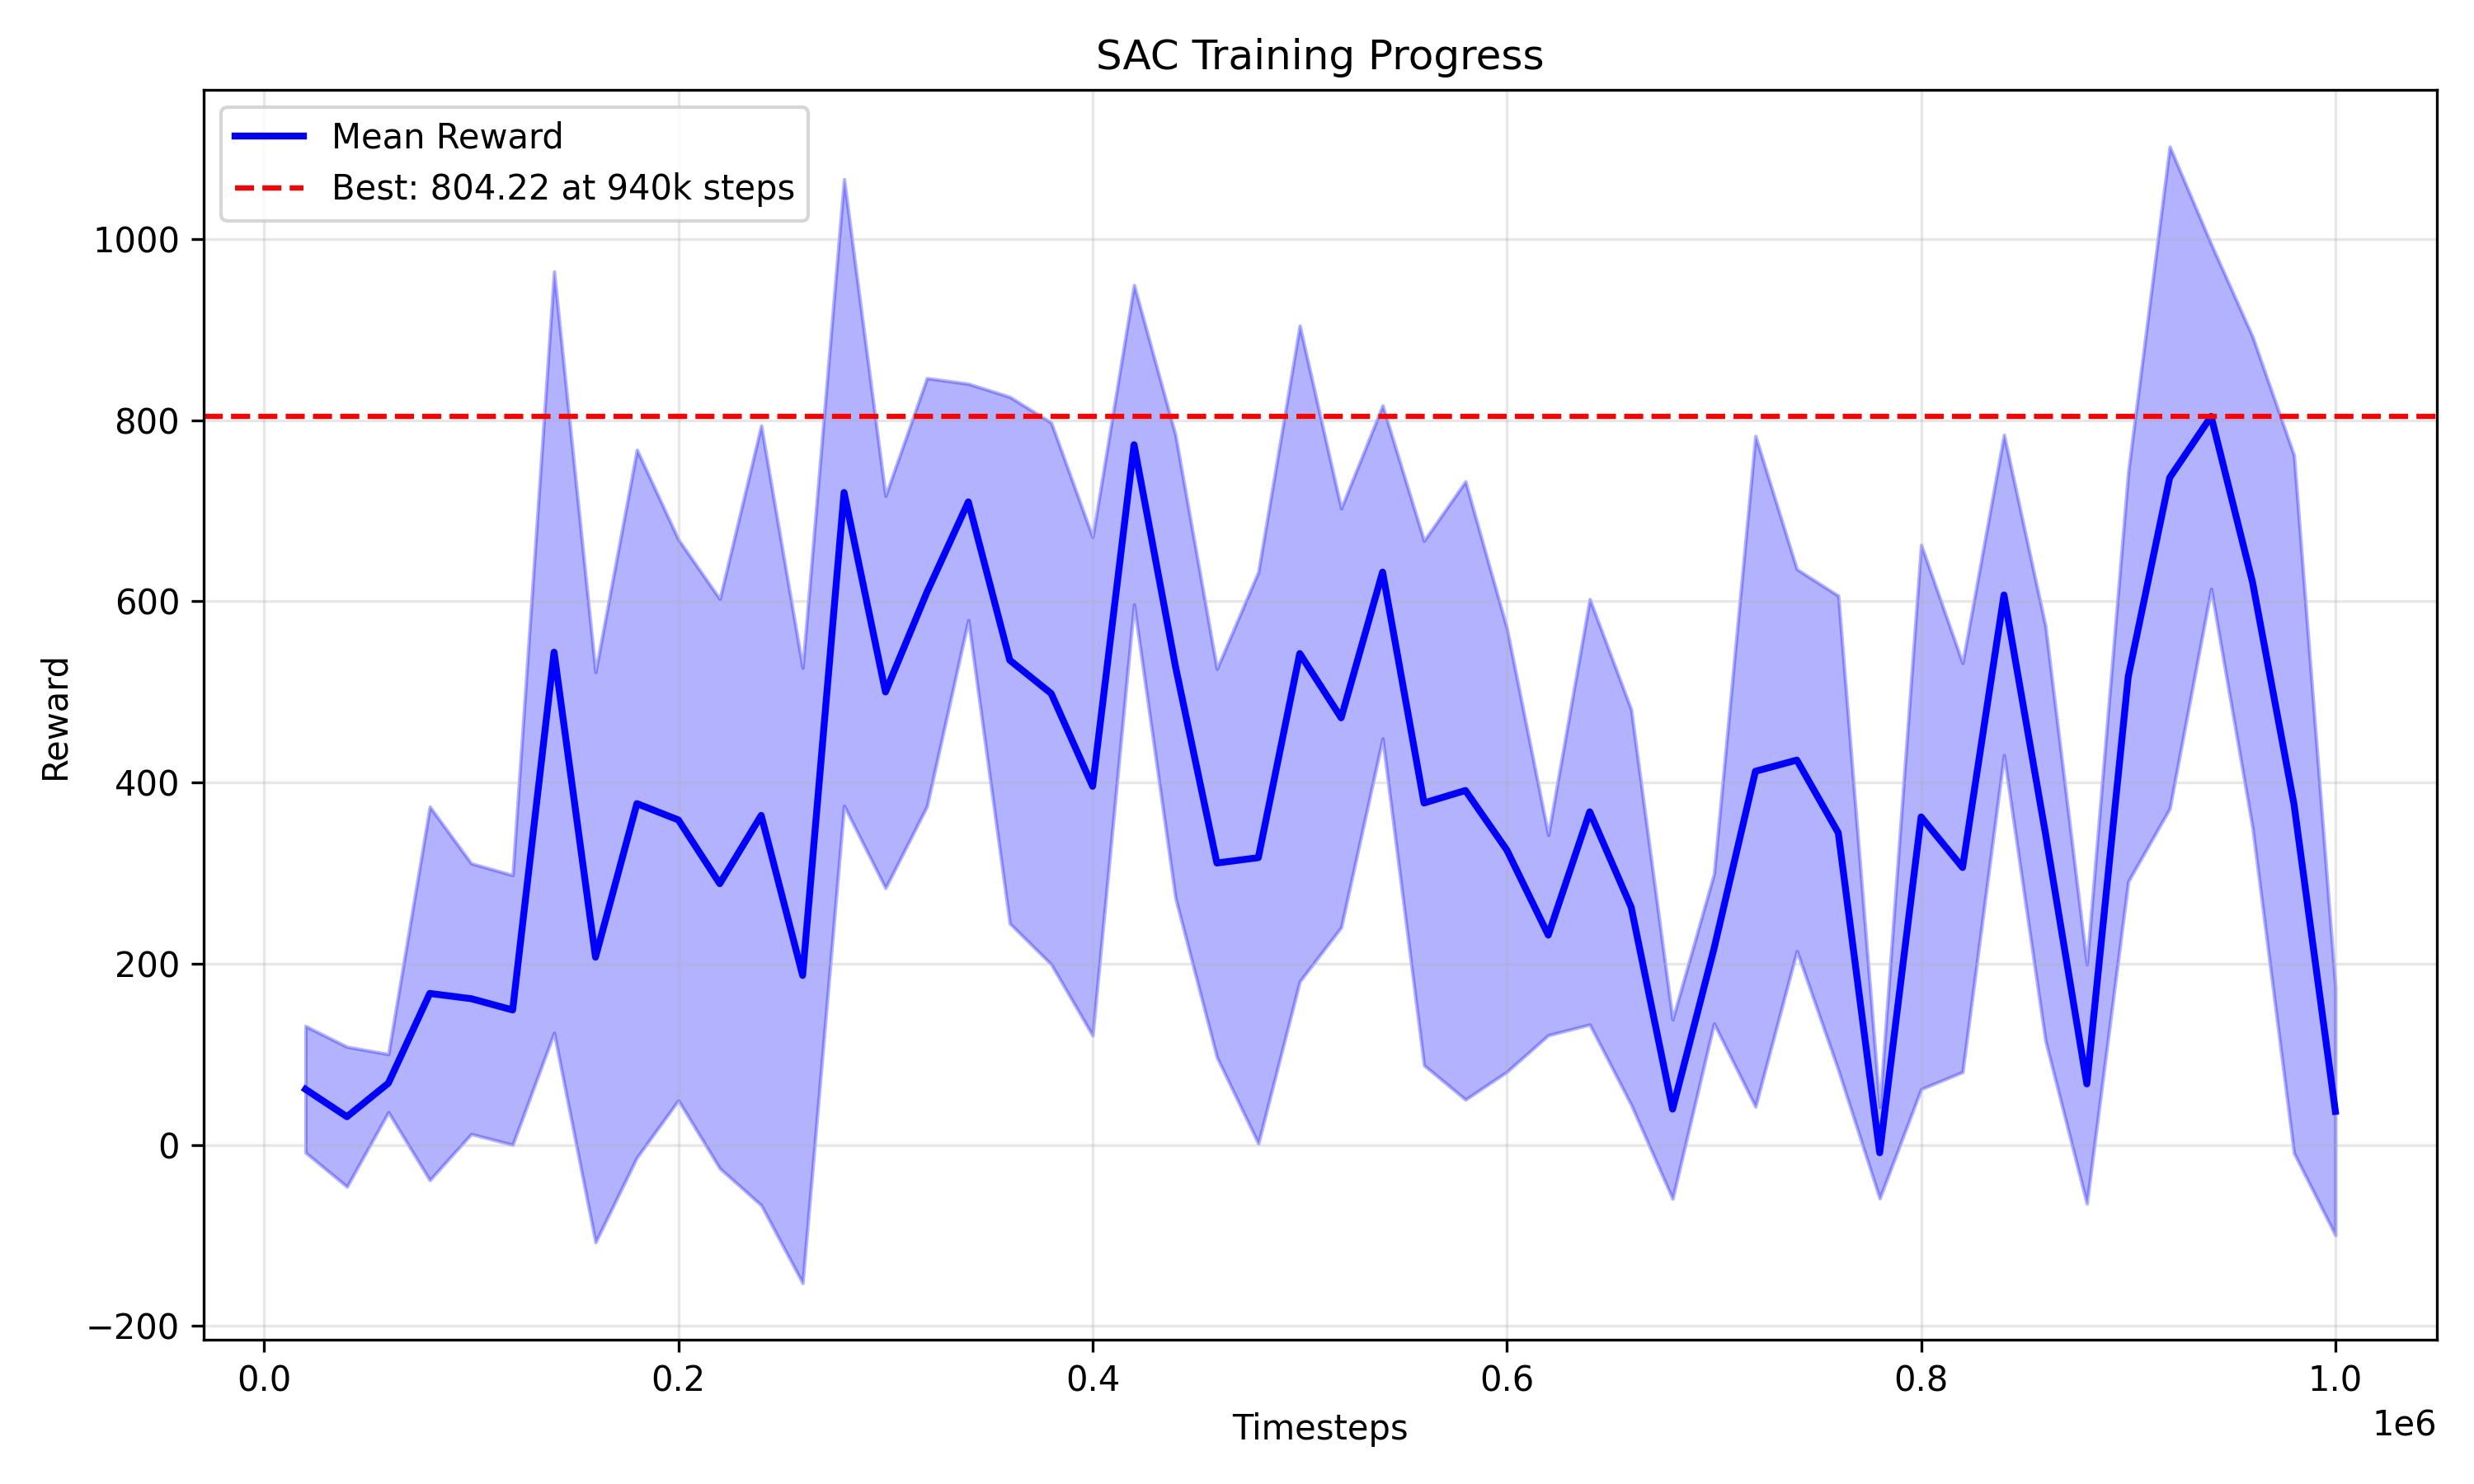
\includegraphics[width=0.75\linewidth]{Writeup/training-progress.png}
    \caption{Training}
    \label{fig:enter-label}
\end{figure}
Figure 5 illustrates the agent's training progression over 1 million timesteps. The blue line shows mean evaluation reward, with the shaded area representing standard deviation. Training exhibited several phases:
\begin{itemize}
    \item Initial rapid improvement (0-200k steps)
    \item Alternating plateaus and breakthroughs (200k-600k steps)
    \item Variable performance with an upward trend (600k-940k steps)
    \item Peak performance of 804.22 at 940k steps (red dashed line)
\end{itemize}

The high variance throughout training reflects the procedurally generated nature of the CarRacing environment, with some tracks being inherently more challenging than others.

\subsection{Behavioral Analysis}
\begin{figure}[H]
    \centering
    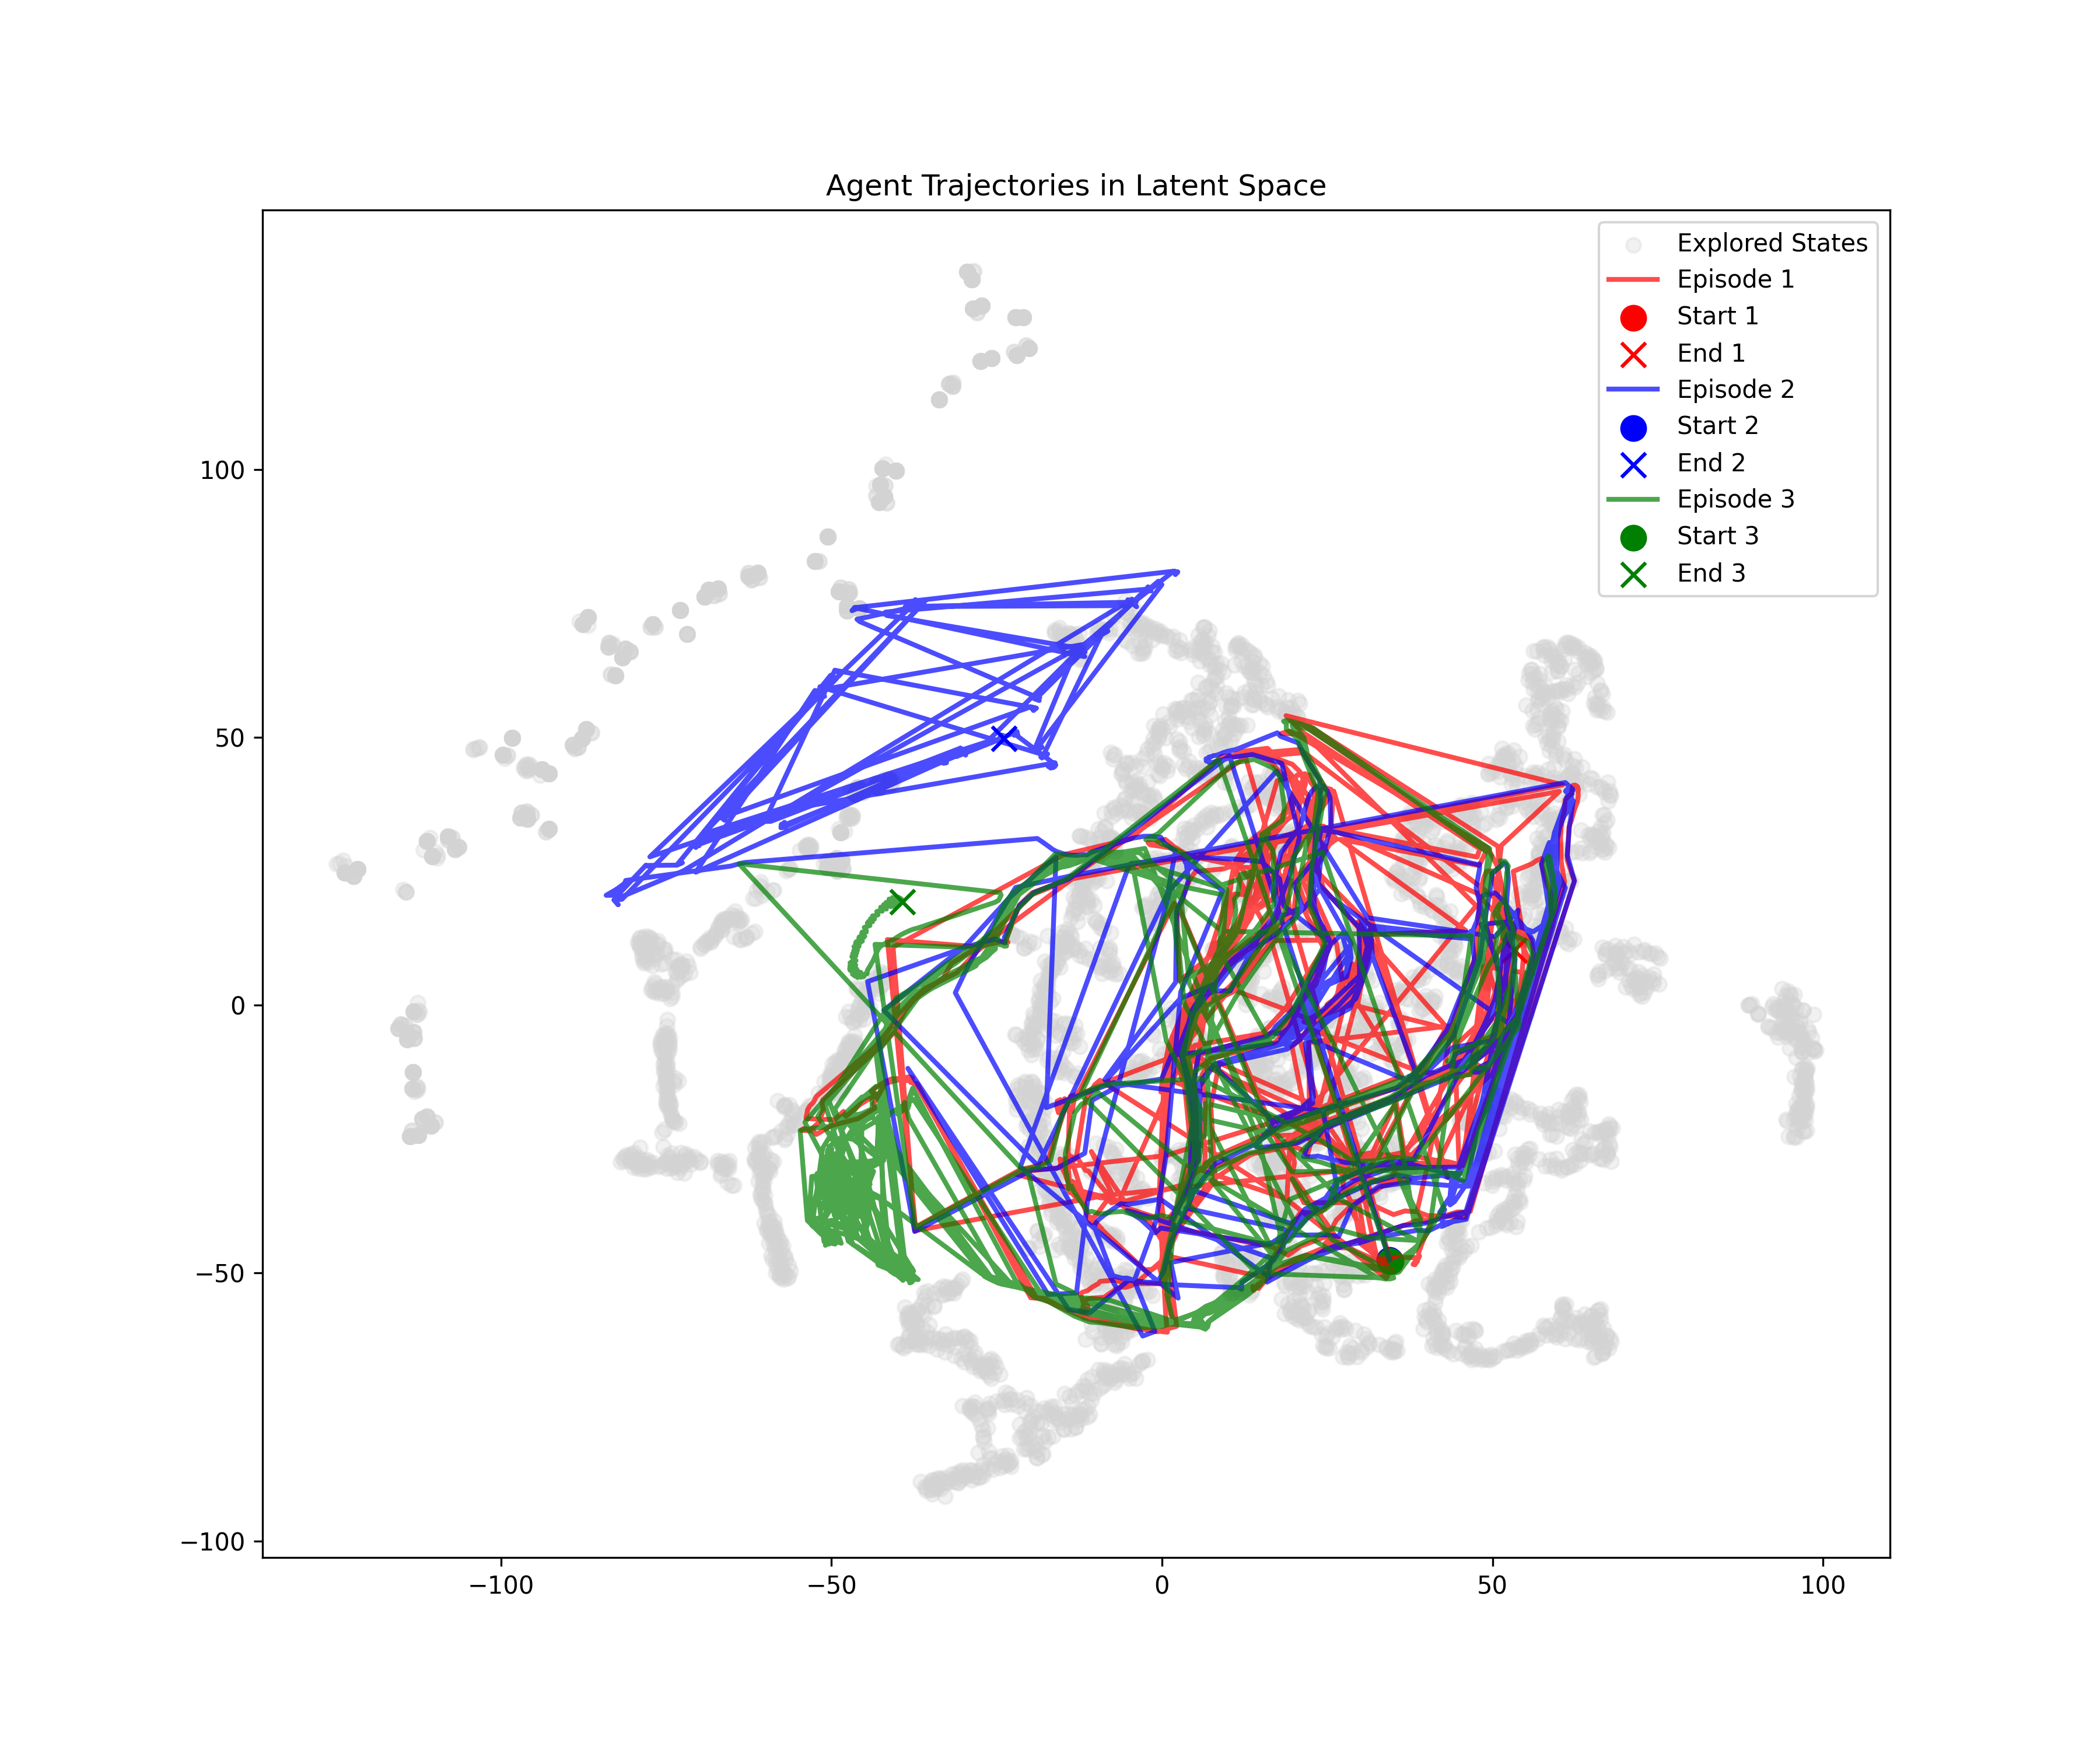
\includegraphics[width=0.75\linewidth]{Writeup/train-visualization.png}
    \caption{Trajectory Visualization}
    \label{fig:enter-label}
\end{figure}
Figure 6 visualizes agent trajectories through the latent space during three complete episodes. The colored lines (red, blue, green) show the agent's path through state space, with gray dots representing previously explored states. These trajectories reveal:
\begin{itemize}
    \item Cyclic patterns corresponding to lap completion
    \item Shared regions across episodes indicating consistent driving strategies
    \item Occasional deviations representing adaptive responses to track variations
\end{itemize}

The trajectories demonstrate that despite being trained in a mere 2D latent space, the agent develops coherent, structured driving behavior that adapts to different track configurations while maintaining a consistent overall strategy.

\subsection{Behavioral Clustering}
\begin{figure}
    \centering
    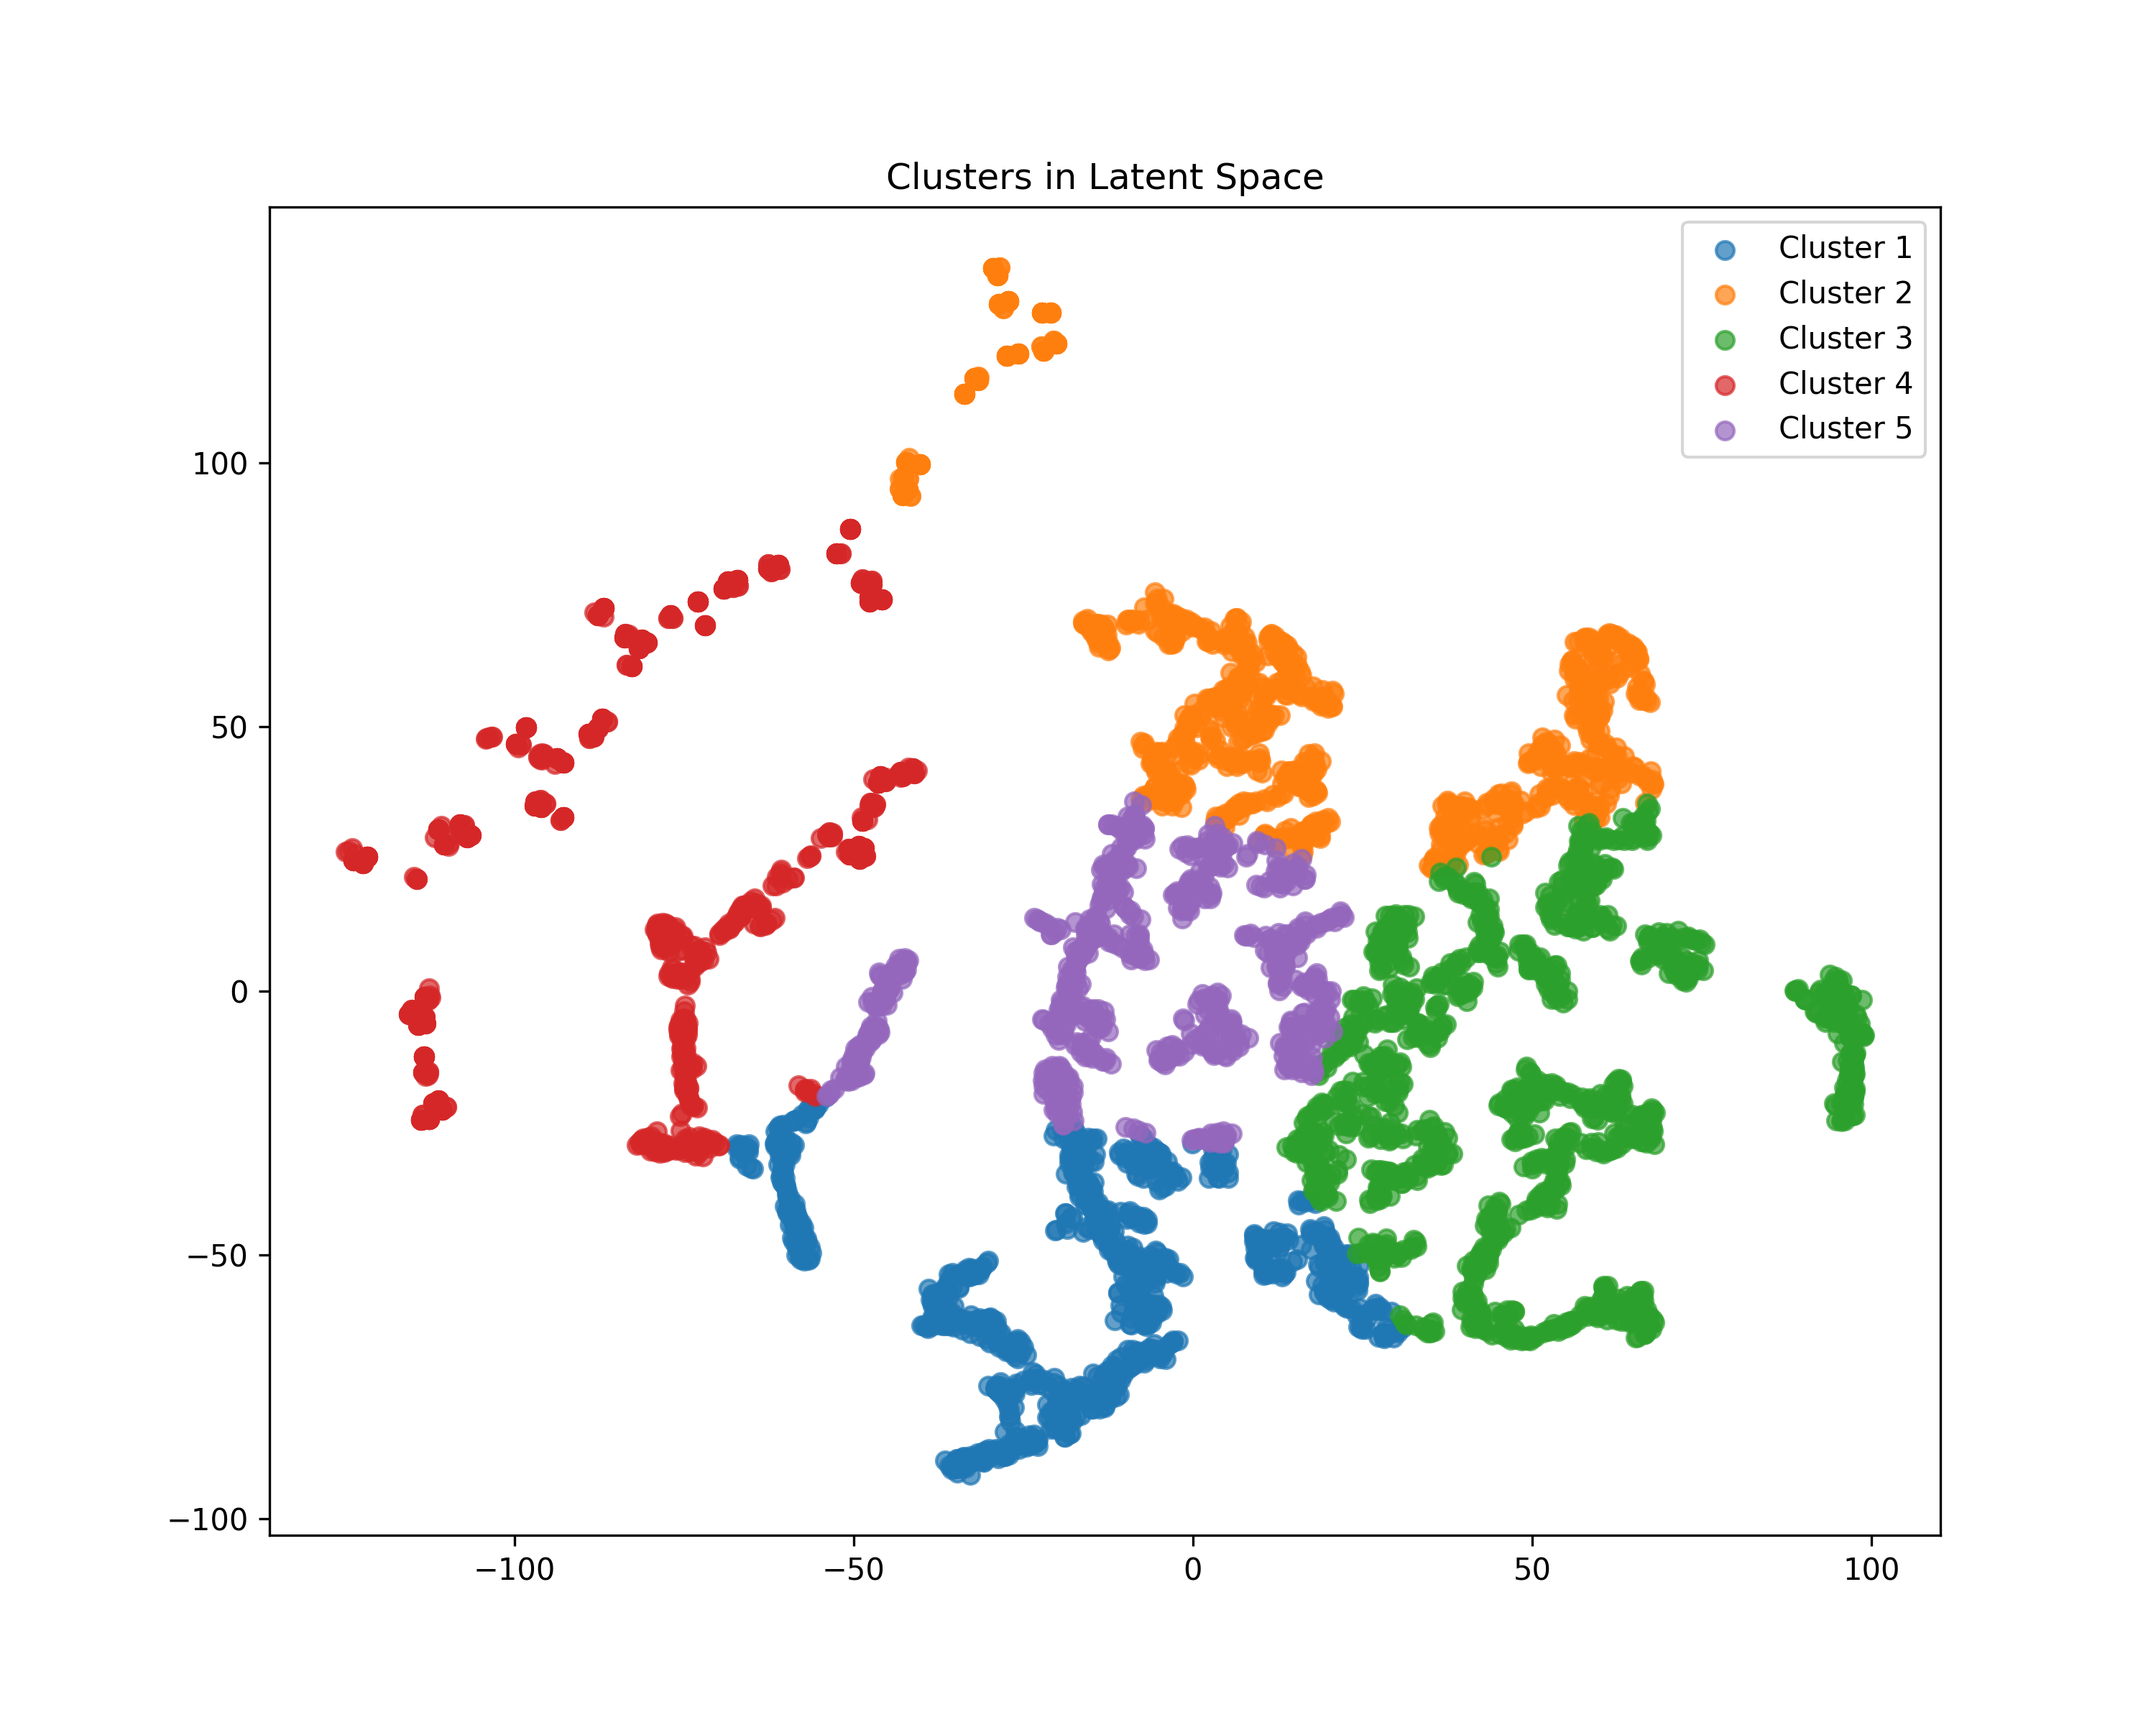
\includegraphics[width=0.5\linewidth]{Writeup/cluster.png}
    \caption{Clustering Analysis}
    \label{fig:enter-label}
\end{figure}
Figure 7 presents the results of K-means clustering (k=5) on states visited by the agent, revealing distinct behavioral modes:
\begin{itemize}
    \item Cluster 1 (Blue): Left turning maneuvers (average steering: -0.543) with high acceleration (0.792)
    \item Cluster 2 (Orange): Right turning maneuvers (average steering: 0.533) with moderate acceleration (0.548)
    \item Cluster 3 (Green): Nearly straight driving (average steering: -0.141) with lower acceleration (0.463)
    \item Cluster 4 (Red): Moderate left turns (average steering: -0.428) with high acceleration (0.854) and significant braking (0.828), likely representing controlled cornering
    \item Cluster 5 (Purple): Mild course corrections (average steering: -0.115) with steady acceleration (0.738)
\end{itemize}

This clustering provides an interpretable taxonomy of the agent's behavioral repertoire, demonstrating how it specializes actions for different driving scenarios.

\subsection{State-Action Relationships}
Figure 8 visualizes the t-SNE embedding of states colored by different attributes. The top-left plot (steering) shows clear separation between left-steering (blue) and right-steering (red) regions. The top-right plot (acceleration) reveals varying acceleration intensity across different state regions, with highest values (yellow) in straightaway sections. The bottom-left plot (Q-value) shows relatively uniform value estimates across the state space, while the bottom-right plot (reward) displays predominantly positive rewards with subtle variations in magnitude.
\begin{figure}[H]
    \centering
    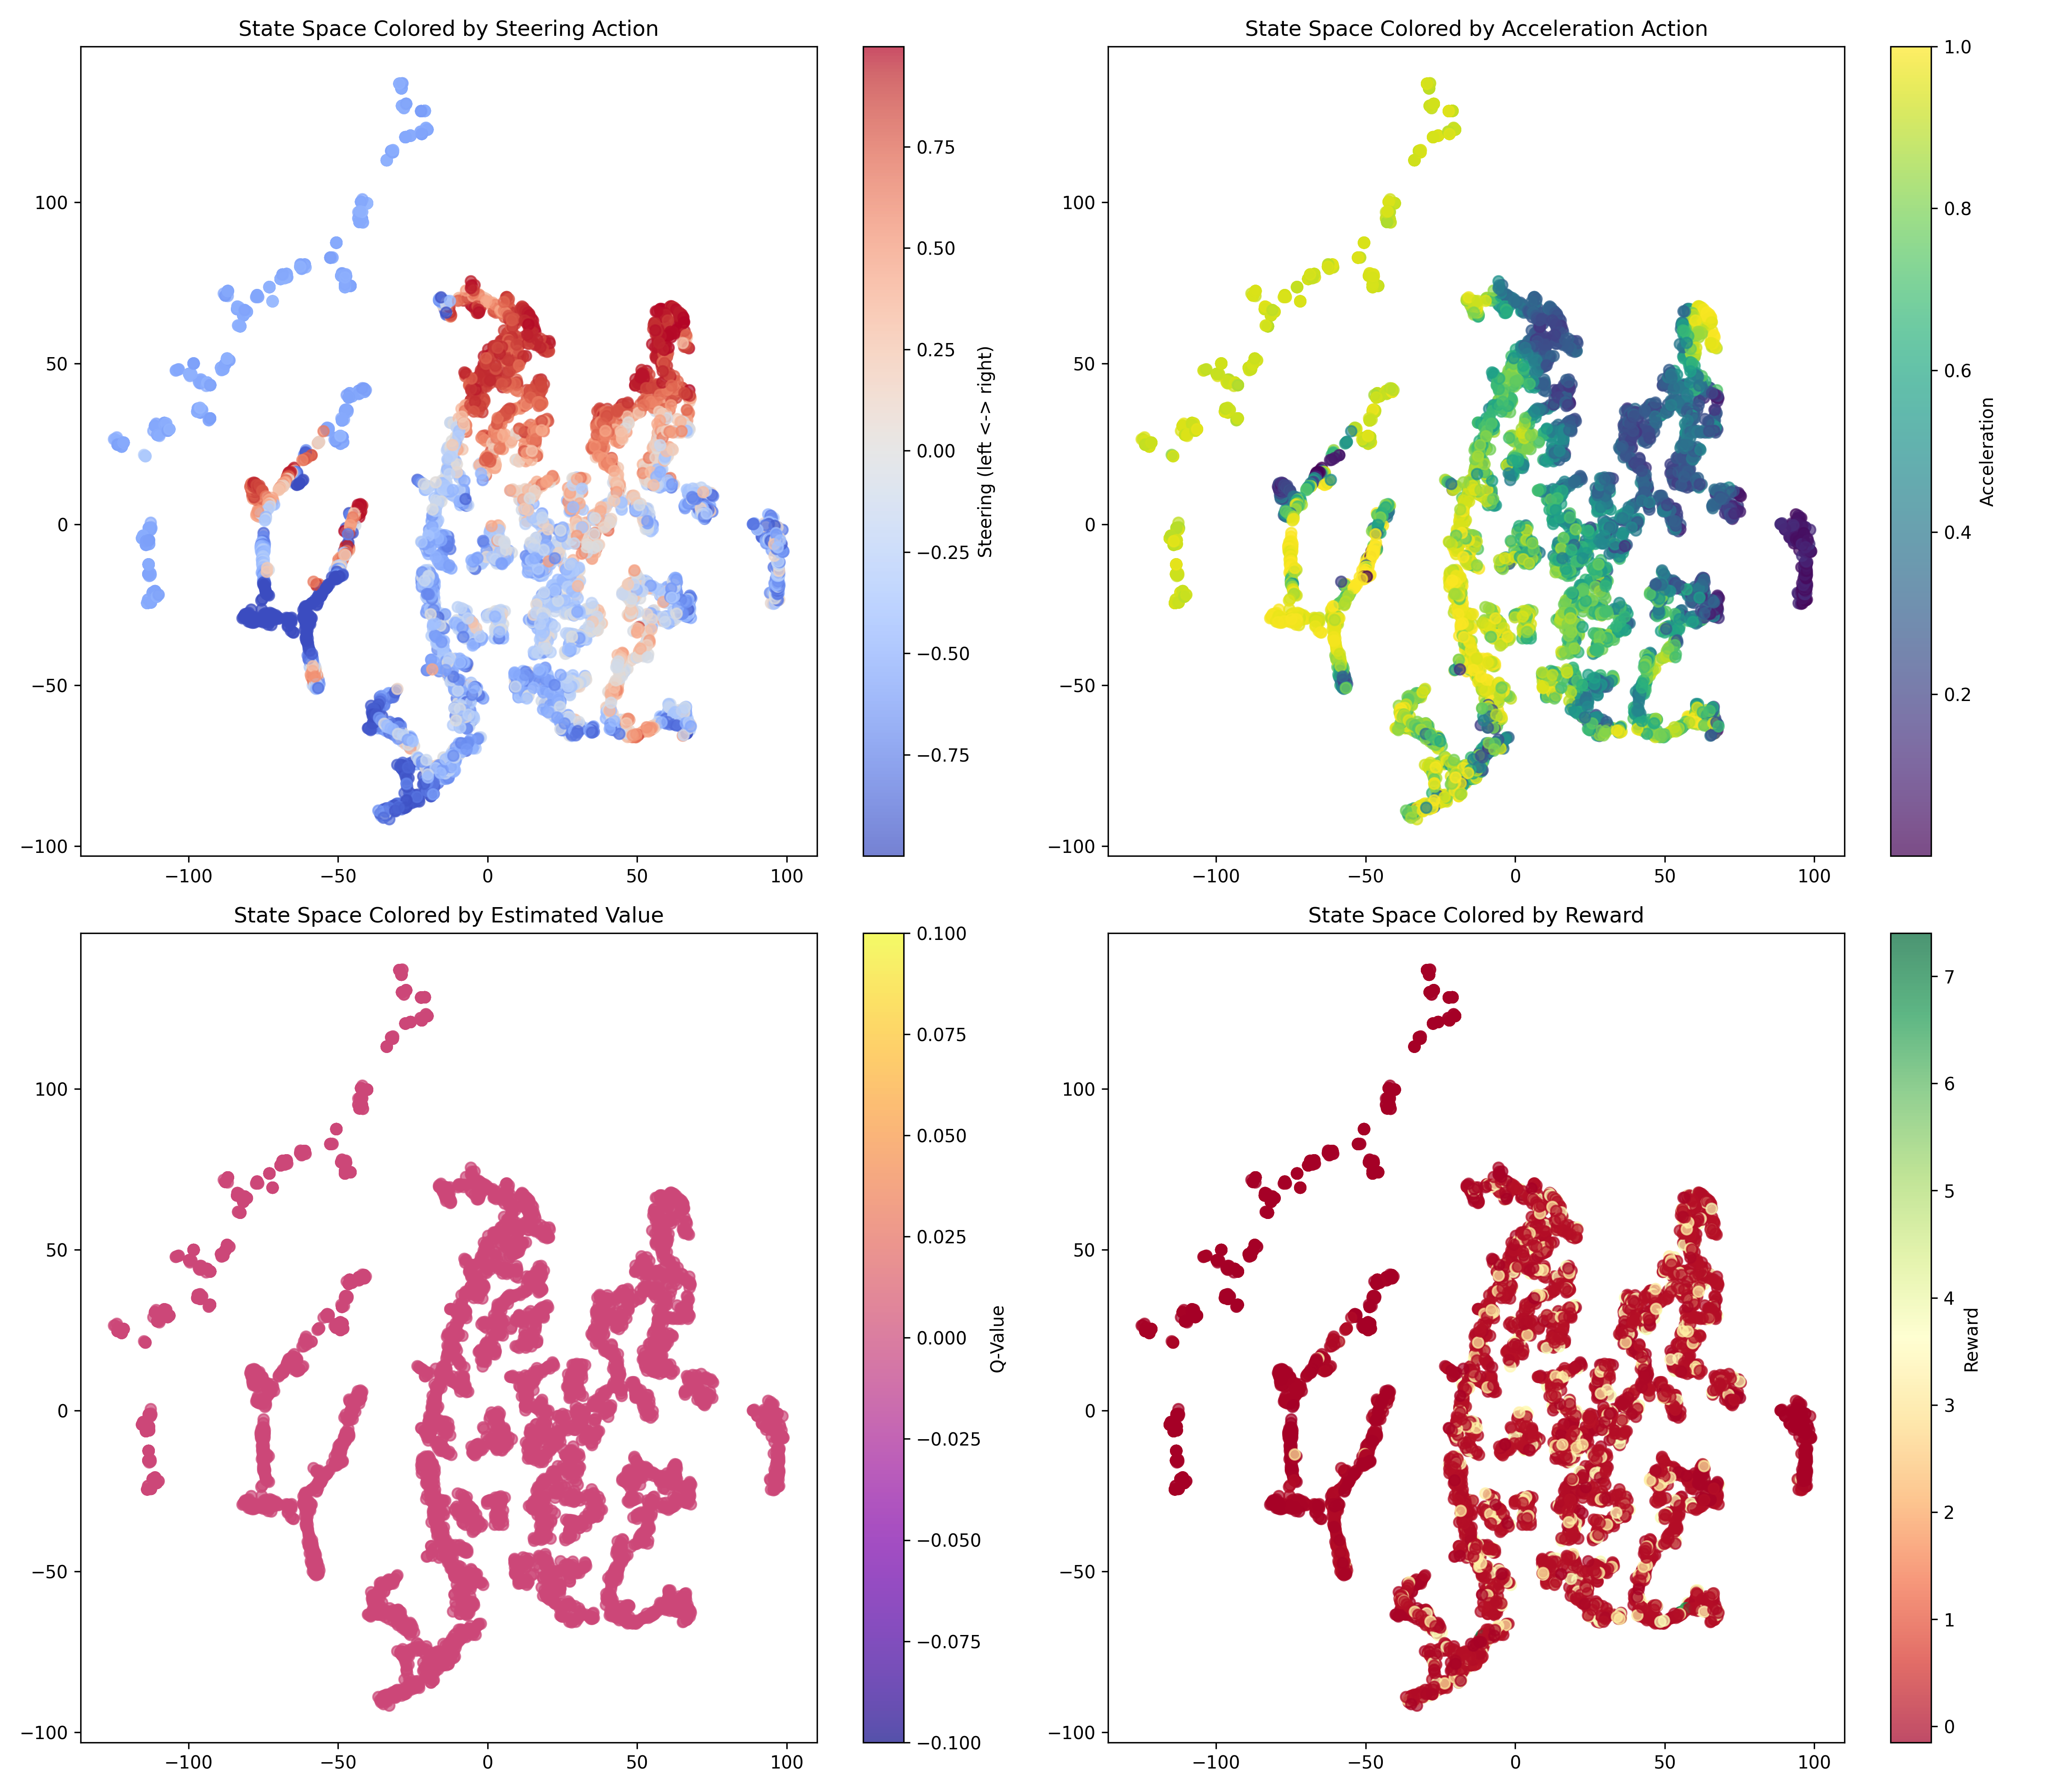
\includegraphics[width=0.75\linewidth]{Writeup/tsne.png}
    \caption{t-SNE Embeddings}
    \label{fig:enter-label}
\end{figure}

10These visualizations reveal logical relationships between states and actions, confirming that the agent has learned appropriate action mappings across the state space. The clear structure in these relationships demonstrates that despite the extreme dimensionality reduction, the agent has developed a coherent and interpretable driving policy.
\section{Conclusion and Future Work}

\subsection{Conclusion}

Our research demonstrates that effective explainability in reinforcement learning can be achieved through dimensionality reduction and visualization of the agent's latent state space. By compressing high-dimensional visual inputs to just two dimensions using a VAE, we created an interpretable representation that enabled both effective policy learning and comprehensive visualization of the agent's decision-making process.

The experimental results show that our approach successfully balances performance and explainability. The agent achieved impressive rewards (average $997.43 \pm 64.79$) while maintaining interpretability through various visualization techniques. The policy vector fields, trajectory analysis, and behavioral clustering provide complementary perspectives on the agent's behavior, revealing how it navigates the driving task through specialized behavioral modes.

Our work challenges the common assumption that deep reinforcement learning systems must function as black boxes. By designing the architecture with explainability as a primary consideration rather than as an afterthought, we created a system that is both high-performing and transparent. This approach represents a significant step toward more trustworthy AI systems that can be deployed in safety-critical domains.

\subsection{Future Work}

While our approach successfully demonstrates explainable RL through latent space visualization, several promising directions for future work remain:

\begin{itemize}
    \item \textbf{Temporal Dynamics:} Our current approach focuses primarily on spatial features but could be extended to explicitly model temporal dynamics. Incorporating recurrent elements or predictive modeling could enhance the agent's ability to anticipate upcoming track features and plan accordingly.
    
    \item \textbf{Complex Environments:} Testing the approach in more realistic driving scenarios with obstacles, other vehicles, varying weather conditions, and more complex rules would assess its scalability to real-world autonomous driving systems.
\end{itemize}

By pursuing these directions, future research can build upon our framework to create even more capable, robust, and transparent reinforcement learning systems that bridge the gap between performance and explainability.

\begin{thebibliography}{00}
\bibitem{b1} G. Eason, B. Noble, and I. N. Sneddon, ``On certain integrals of Lipschitz-Hankel type involving products of Bessel functions,'' Phil. Trans. Roy. Soc. London, vol. A247, pp. 529--551, April 1955.
\bibitem{b2} J. Clerk Maxwell, A Treatise on Electricity and Magnetism, 3rd ed., vol. 2. Oxford: Clarendon, 1892, pp.68--73.
\bibitem{b3} I. S. Jacobs and C. P. Bean, ``Fine particles, thin films and exchange anisotropy,'' in Magnetism, vol. III, G. T. Rado and H. Suhl, Eds. New York: Academic, 1963, pp. 271--350.
\bibitem{b4} K. Elissa, ``Title of paper if known,'' unpublished.
\bibitem{b5} R. Nicole, ``Title of paper with only first word capitalized,'' J. Name Stand. Abbrev., in press.
\bibitem{b6} Y. Yorozu, M. Hirano, K. Oka, and Y. Tagawa, ``Electron spectroscopy studies on magneto-optical media and plastic substrate interface,'' IEEE Transl. J. Magn. Japan, vol. 2, pp. 740--741, August 1987 [Digests 9th Annual Conf. Magnetics Japan, p. 301, 1982].
\bibitem{b7} M. Young, The Technical Writer's Handbook. Mill Valley, CA: University Science, 1989.
\end{thebibliography}
\vspace{12pt}

\end{document}
